\subsection{FPT Shop}
\begin{figure}[H]
    \centering
    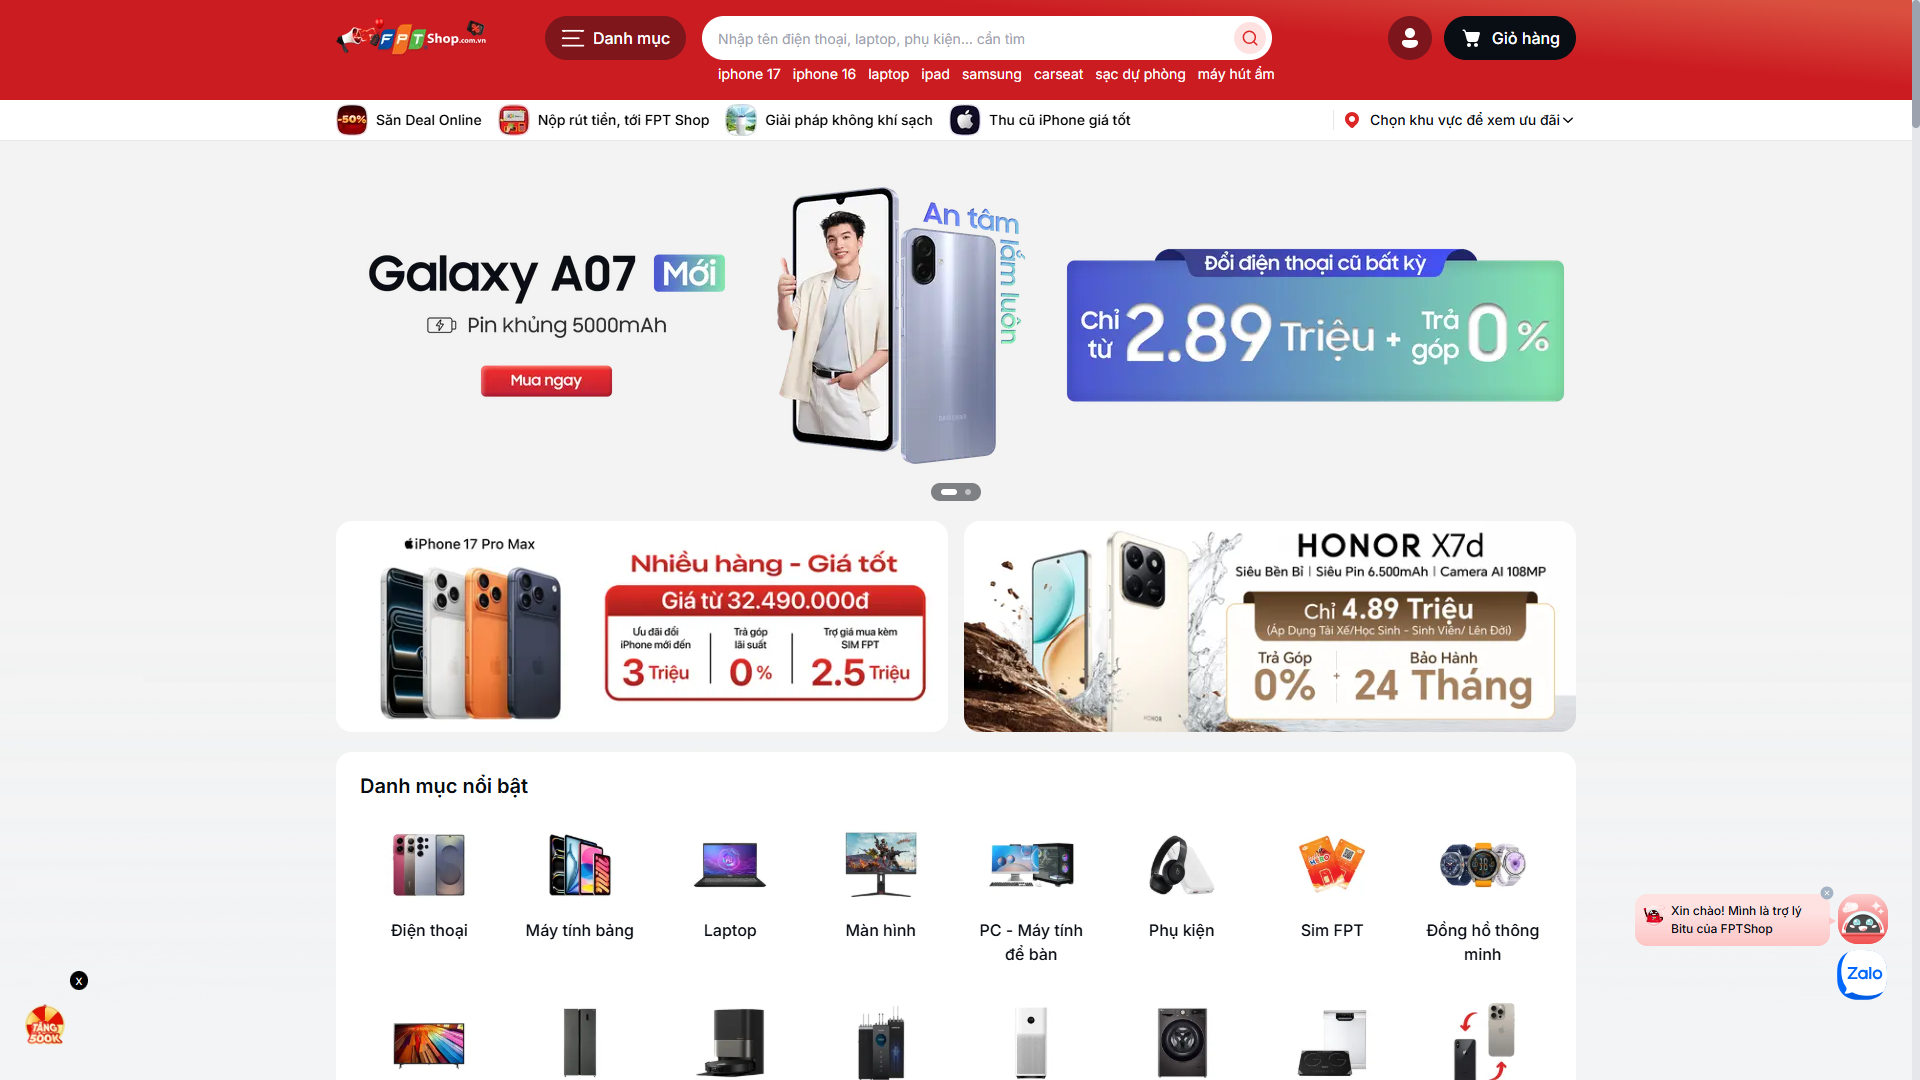
\includegraphics[width=\textwidth]{images/chap2/fpt.png}
    \vspace{0.5cm}
    \caption{Trang chủ của FPT Shop}
\end{figure}

FPT Shop là thương hiệu bán lẻ thiết bị công nghệ thuộc Tập đoàn FPT, với mạng lưới cửa hàng rộng khắp và nền tảng thương mại điện tử tích hợp mạnh mẽ. Website của FPT Shop chú trọng trải nghiệm người dùng, hỗ trợ trả góp, khuyến mãi và dịch vụ hậu mãi, đồng thời ứng dụng công nghệ AI trong tư vấn, hỗ trợ khách hàng.

\textbf{Tính năng nổi bật:}
\begin{itemize}
    \item Hệ thống tìm kiếm và lọc sản phẩm mạnh, hiển thị nhiều biến thể sản phẩm và cho phép so sánh cơ bản.
    \item Hỗ trợ trả góp đa dạng với thông tin minh bạch về lãi suất và các tùy chọn thanh toán.
    \item Ứng dụng di động cung cấp thông tin khuyến mãi, voucher và tích điểm khách hàng thân thiết.
\end{itemize}

FPT Shop sở hữu nền tảng công nghệ hiện đại với khả năng đồng bộ tốt giữa kênh bán hàng trực tuyến và hệ thống cửa hàng vật lý, mang lại trải nghiệm mua sắm liền mạch cho người dùng. Website cung cấp đầy đủ các chức năng như tra cứu sản phẩm, xem thông tin chi tiết, so sánh và đặt hàng trực tuyến, đáp ứng hiệu quả nhu cầu mua sắm của khách hàng.

Tuy nhiên, hệ thống hiện chưa tích hợp trợ lý ảo hoặc chatbot thông minh trên nền tảng web để hỗ trợ người dùng trong quá trình tương tác. Việc hỗ trợ khách hàng chủ yếu vẫn dựa vào các kênh truyền thống như tổng đài hoặc tư vấn viên trực tuyến. Cách tiếp cận này giúp đảm bảo độ chính xác trong phản hồi, nhưng đồng thời làm hạn chế khả năng tự động hóa và phản hồi nhanh, đặc biệt khi số lượng người dùng tăng cao.

Bên cạnh đó, việc thiếu một hệ thống trợ lý ảo cũng khiến trải nghiệm người dùng vẫn mang tính thụ động, phụ thuộc vào thao tác tìm kiếm và điều hướng thủ công. Điều này cho thấy tiềm năng ứng dụng trí tuệ nhân tạo trong việc hỗ trợ tư vấn, so sánh sản phẩm và giải đáp thắc mắc vẫn chưa được khai thác hiệu quả trong hệ thống.